\documentclass[conference]{IEEEtran}

% ---- Packages ----
\usepackage{cite}
\usepackage{amsmath,amssymb}
\usepackage{graphicx}
\usepackage{tikz}
\usepackage{ifthen}
\usepackage{booktabs}
\usepackage{hyperref}
\usepackage{newtxtext,newtxmath} % Times系フォント

% ---- Metadata ----
\title{Historical Case Study on Ti Silicide (TiSi\textsubscript{2}) Reliability Issues in Legacy CMOS Nodes}

\author{
\IEEEauthorblockN{Shinichi Samizo}
\IEEEauthorblockA{Independent Semiconductor Researcher\\
Project Design Hub, Samizo-AITL\\
\textit{Email:} \href{mailto:shin3t72@gmail.com}{shin3t72@gmail.com}\quad
\textit{GitHub:} \href{https://github.com/Samizo-AITL}{Samizo-AITL}}
}

\begin{document}
\maketitle

% ---------- Abstract ----------
\begin{abstract}
This paper analyzes a historical failure case related to Ti silicide (TiSi\textsubscript{2}) phase transition instability at the 0.25\,µm CMOS node. 
The incomplete C49$\rightarrow$C54 transformation, coupled with boron absorption, caused localized high-resistance spots that directly reduced SRAM yield. 
The case illustrates how process optimization and empirical feedback cycles became indispensable in semiconductor development under cost and market pressure.
\end{abstract}

% ---------- 1. Introduction ----------
\section{Introduction}
Around 2000, passive-matrix monochrome panels were being replaced by TFT-LCDs, driving demand for large-scale SRAM and mixed-signal logic in driver ICs. 
Under market pressure from Korean and Taiwanese competitors, some manufacturers attempted to extend the 0.25\,µm process instead of migrating to 0.18\,µm, in order to reduce cost. 
This historical decision revealed vulnerabilities when Ti salicide process instabilities degraded yield.

% ---------- 2. Technical Background ----------
\section{Technical Background}
TiSi\textsubscript{2} was widely adopted for its low resistivity. 
However, the silicide undergoes a phase transition from metastable C49 to stable C54 during rapid thermal annealing (RTA). 
If the transition is incomplete, residual C49 grains act as high-resistance regions. 
Furthermore, boron absorption into TiSi\textsubscript{2} aggravated resistance fluctuation, directly manifesting as random SRAM bit failures.

% ---------- 3. Failure Analysis ----------
\section{Failure Analysis}
The yield impact was confirmed through SRAM testing. 
Without redundancy, single-bit random defects directly caused device rejection. 
Failure localization pointed to silicide regions at transistor contacts, with boron diffusion paths accelerating local resistivity increase.

\begin{figure}[t]
\centering
% --- Guard for missing external figure ---
\newcommand{\SRAMYieldFig}{}
\IfFileExists{figures/fig_sram_yield.pdf}{\renewcommand{\SRAMYieldFig}{figures/fig_sram_yield.pdf}}{}
\IfFileExists{figures/fig_sram_yield.png}{\renewcommand{\SRAMYieldFig}{figures/fig_sram_yield.png}}{}

\ifthenelse{\equal{\SRAMYieldFig}{}}
{%
  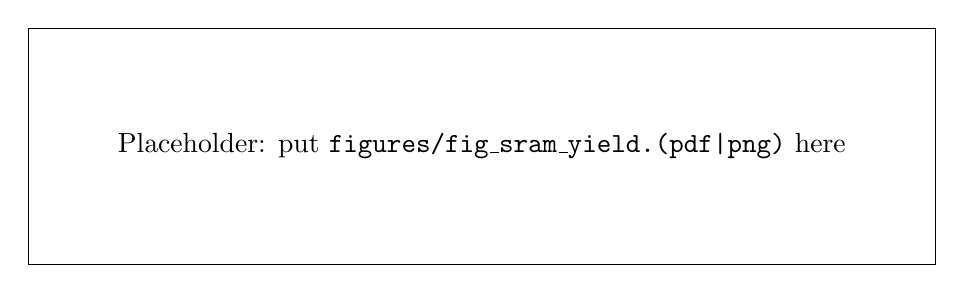
\begin{tikzpicture}
    \node[draw,minimum width=0.95\linewidth,minimum height=3cm,align=center]
      {Placeholder: put \texttt{figures/fig\_sram\_yield.(pdf|png)} here};
  \end{tikzpicture}
}
{%
  \includegraphics[width=0.95\linewidth]{\SRAMYieldFig}
}
\caption{Illustrative yield sensitivity (Poisson model) with/without redundancy.}
\label{fig:sram_yield}
\end{figure}

% ---------- 4. Review and Limitations ----------
\section{Design Review Limitations}
Design reviews (DR) could only verify rule compliance and formal specifications. 
They failed to predict scalability risks arising from incomplete silicide phase transformation. 
This case shows that DR without continuous empirical feedback was insufficient.

% ---------- 5. Countermeasures ----------
\section{Countermeasures}
\subsection{Provisional Measures}
Etch profiles were adjusted to slightly undercut sidewalls, ensuring sufficient separation between halo implants and active regions. 
This measure temporarily improved yield.

\subsection{Permanent Measures}
RTA conditions were optimized to stabilize C54 phase formation. 
However, this changed device parameters, requiring re-characterization of process-device models.

% ---------- 6. Educational Application ----------
\section{Educational Application}
\subsection{Teaching Materials}
\begin{itemize}
  \item Cause-effect diagrams linking process $\rightarrow$ defect $\rightarrow$ yield
  \item Comparative tables: 0.25\,µm vs 0.18\,µm (technology vs cost)
  \item Exercises: process fix vs redundancy adoption
\end{itemize}

\subsection{Universality}
Trade-offs between technical stability and economic pressure remain relevant today. 
Similar cases exist in re-use of 28\,nm FD-SOI or 40\,nm BCD. 

% ---------- 7. Conclusion ----------
\section{Conclusion}
This historical case demonstrates that residual risks remain in legacy nodes. 
Yield degradation due to incomplete silicide phase transition highlighted the inseparability of process optimization and empirical feedback. 
The educational value lies in integrating such case studies into semiconductor engineering curricula.

% ---------- References ----------
\begin{thebibliography}{99}

\bibitem{Sze}
S. M. Sze and K. K. Ng, \emph{Physics of Semiconductor Devices}, 3rd ed. Hoboken, NJ, USA: Wiley, 2007.

\bibitem{Wolf}
S. Wolf and R. N. Tauber, \emph{Silicon Processing for the VLSI Era, Volume 1: Process Technology}. Sunset Beach, CA, USA: Lattice Press, 1986.

\bibitem{Colinge}
J.-P. Colinge, \emph{Silicon-on-Insulator Technology: Materials to VLSI}, 3rd ed. Springer, 2004.

\bibitem{ITRS}
International Technology Roadmap for Semiconductors (ITRS), ``Process Integration, Devices, and Structures,'' 2001.

\bibitem{Takeda1994}
E. Takeda, C. Y. Yang, and A. S. Grove, ``Silicide technology for ULSI applications,'' \emph{IEEE Transactions on Electron Devices}, vol. 41, no. 12, pp. 2133--2141, Dec. 1994.

\bibitem{Chang1996}
J. P. Chang and A. J. Steckl, ``Titanium silicide formation and stability in submicron CMOS technology,'' \emph{Journal of Applied Physics}, vol. 79, no. 9, pp. 4356--4364, 1996.

\end{thebibliography}

% ---------- Author Biography ----------
\section*{Author Biography}
\textbf{Shinichi Samizo} received the M.S. degree in Electrical and Electronic Engineering from Shinshu University, Japan. 
He worked at Seiko Epson Corporation on semiconductor memory and mixed-signal device development and contributed to inkjet MEMS actuators and PrecisionCore printhead technology. 
He is currently an independent semiconductor researcher focusing on process/device education, memory architecture, and AI system integration. \\
\emph{Contact:} \href{mailto:shin3t72@gmail.com}{shin3t72@gmail.com}\quad
\emph{GitHub:} \href{https://github.com/Samizo-AITL}{Samizo-AITL}.

\end{document}
